\documentclass[11pt,letterpaper]{article}

\usepackage[margin=0.85in]{geometry}
\usepackage{amsmath,amssymb}
\usepackage{booktabs}
\usepackage{graphicx}
\usepackage{xcolor}
\usepackage{hyperref}
\usepackage{enumitem}
\usepackage{multicol}
\usepackage{tikz}
\usepackage{pgfplots}
\pgfplotsset{compat=1.18}
\usetikzlibrary{arrows.meta,positioning,calc}
\usepackage{parskip}
\usepackage{microtype}

\hypersetup{colorlinks=true,linkcolor=blue!60!black,urlcolor=blue!60!black}

\setlength{\parskip}{4pt}
\setlength{\parindent}{0pt}

\begin{document}

% ---- Header ----
{\Large\bfseries Learned Rosters Under Pressure: Roster Optimization via\\
Graph-Scored Search and Adversarial Evaluation}

\vspace{0.5em}
{\bfseries Luke Blommesteyn\,$^1$ \quad Jaden Majumdar\,$^2$}\\[0.2em]
$^1$University of Western Ontario \quad \texttt{lblommes@uwo.ca}\\
$^2$University of Toronto \quad \texttt{jaden.majumdar@mail.utoronto.ca}\\
{\small\url{https://github.com/lblommesteyn/groupWAR}}

\vspace{0.4em}
{\color{gray!60}\hrule}
\vspace{0.6em}

% ---- Abstract ----
\textbf{Abstract.}
We formulate national-team roster selection as a formal optimization
problem combining learned scoring with adversarial game theory.
A Graph Convolutional Network (GCN), trained on 6{,}100+ historical
game-level lineups, scores the win probability of any candidate
roster. Rosters are then evaluated in an adversarial loop: the
opponent selects the best counter-lineup via gradient descent, and the
search maximizes win probability against this counter. The search
phase uses tournament elimination and batched greedy refinement to
navigate the combinatorial space. Two domain-aware design choices are
critical: (1)~\emph{positional quotas} prevent degenerate local
optima (e.g., 10 centers, 0 wings in hockey); (2)~\emph{stochastic
rotation scoring} bridges the 5-on-5 model / 12-player roster
mismatch in basketball. Applied to the 2025 4 Nations Face-Off
(Canada Hockey) and the 2024 Paris Olympics (USA and Canada
Basketball), constrained rosters recover many core national-team
selections while maintaining internal coherence (all positive
Wins Above Replacement).

\vspace{0.2em}

% ---- Pipeline figure ----
\begin{figure}[h]
\centering
\small
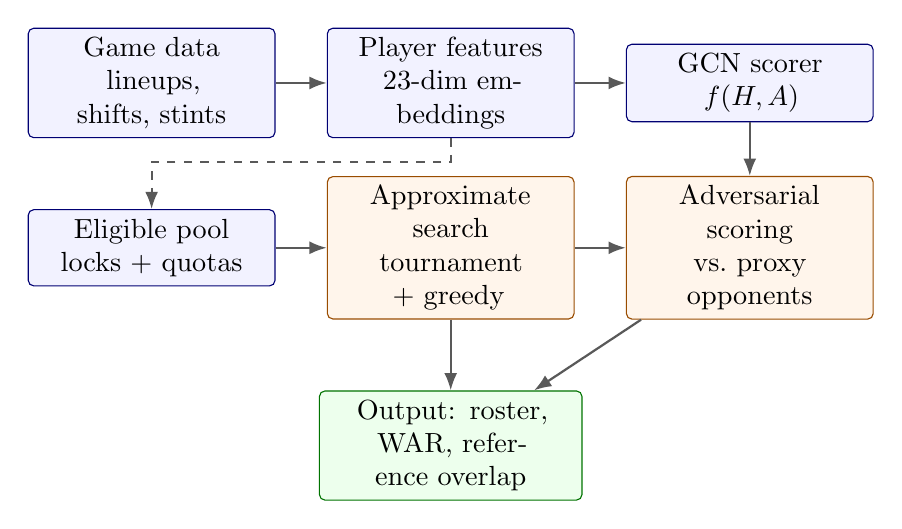
\begin{tikzpicture}[
  box/.style={draw=blue!45!black,fill=blue!5,rounded corners=2pt,
              align=center,text width=2.9cm,minimum height=0.85cm},
  evalbox/.style={draw=orange!60!black,fill=orange!8,rounded corners=2pt,
                  align=center,text width=2.9cm,minimum height=0.85cm},
  outbox/.style={draw=green!45!black,fill=green!7,rounded corners=2pt,
                 align=center,text width=3.1cm,minimum height=0.85cm},
  arrow/.style={-{Latex[length=2.2mm]},thick,draw=gray!70!black},
  node distance=0.65cm and 0.65cm
]
  \node[box] (data) {Game data\\lineups, shifts, stints};
  \node[box, right=of data] (features) {Player features\\23-dim embeddings};
  \node[box, right=of features] (gcn) {GCN scorer\\$f(H,A)$};
  \node[box, below=0.9cm of data] (pool) {Eligible pool\\locks + quotas};
  \node[evalbox, right=of pool] (search) {Approximate search\\tournament + greedy};
  \node[evalbox, right=of search] (stack) {Adversarial scoring\\vs.\ proxy opponents};
  \node[outbox, below=0.9cm of search] (final) {Output: roster,\\WAR, reference overlap};
  \draw[arrow](data)--(features);
  \draw[arrow](features)--(gcn);
  \draw[arrow](pool)--(search);
  \draw[arrow](gcn)--(stack);
  \draw[arrow](search)--(stack);
  \draw[arrow](stack)--(final);
  \draw[arrow](search)--(final);
  \draw[arrow,dashed](features.south)--++(0,-0.3)-|(pool.north);
\end{tikzpicture}
\caption{End-to-end pipeline. Player embeddings feed a GCN scorer;
  the search uses locks, positional quotas, and adversarial evaluation
  to navigate ${\sim}10^{28}$ candidate rosters down to one.}
\label{fig:pipeline}
\end{figure}

\vspace{0.2em}

% ---- Approach ----
\textbf{Approach.}
Player-seasons are encoded as 23-dimensional feature vectors covering
shot-zone proportions (7 zones), assist-zone features, rate
statistics, TOI, and positional flags. APM is computed separately via
ridge regression and used for player ranking and rotation ordering but
is \emph{not} fed into the GCN, so that a RAPM correlation check
($r=0.81$, $\rho=0.78$, $n=287$) constitutes an independent
validation of the ranking signal. The GCN uses a 6-layer message-passing
architecture with a DeepSet aggregation (permutation-invariant) and an
antisymmetric output head ensuring $f(H,A)=1-f(A,H)$.

The adversarial evaluation runs 100 gradient steps with a 5:1
leader-to-follower update ratio. The leader (our roster) maximizes
win probability; the follower (opponent) minimizes it by re-optimizing
their lineup at each step. This rewards rosters with no exploitable
positional weakness over those with a single dominant unit.

Wins Above Replacement (WAR) is defined as $\text{WAR}_i = \hat{y}(\text{full}) - \hat{y}(\text{lineup}_{\setminus i})$:
the drop in team score when player $i$ is removed. All-positive WAR
is used as a \emph{conditional coherence diagnostic} — if any player
shows negative WAR, the lineup is internally inconsistent.

\newpage

% ---- Results ----
\textbf{Results.}

\smallskip
\textit{Canada Hockey 2025 (4 Nations Face-Off).}
The constrained pipeline (5C / 4L / 3R / 6D, six-defenseman target)
recovers 9 of 13 pre-identified core/reference selections
(McDavid, MacKinnon, Crosby, Makar, Theodore, Doughty, Parayko,
Stone, Reinhart) and assigns positive WAR to all 18 players
(max $+0.0179$, min $+0.0009$). Depth picks (Marchand, Hagel,
Kyrou, Crouse) are established two-way forwards who complement the
elite core.

\smallskip
\textit{Basketball 2024 Paris Olympics.}
Stochastic rotation scoring (10 weighted 5-man samples drawn from
empirical playing-time distributions) bridges the 5-on-5 GCN and the
12-player roster. USA overlaps with 8 of 12 Paris Olympians; Canada
overlaps with 9 of 12.

\vspace{0.3em}
\begin{center}
\small
\begin{minipage}{0.44\textwidth}
  \centering
  \textbf{USA Basketball 2024} \quad (score $= 0.7418$)\\[0.3em]
  \begin{tabular}{rl}
    \toprule
    \# & Player \\ \midrule
    1  & Stephen Curry$^{\star}$ \\
    2  & Jrue Holiday \\
    3  & Jayson Tatum \\
    4  & Donovan Mitchell \\
    5  & LeBron James$^{\star}$ \\
    6  & Kevin Durant$^{\star}$ \\
    7  & Anthony Davis$^{\star}$ \\
    8  & Draymond Green \\
    9  & Jaylen Brown \\
    10 & Bam Adebayo \\
    11 & Jimmy Butler \\
    12 & Tyrese Haliburton \\
    \bottomrule
  \end{tabular}
\end{minipage}%
\hfill
\begin{minipage}{0.44\textwidth}
  \centering
  \textbf{Canada Basketball 2024} \quad (score $= 0.6587$)\\[0.3em]
  \begin{tabular}{rl}
    \toprule
    \# & Player \\ \midrule
    1  & SGA$^{\star}$ \\
    2  & Jamal Murray$^{\star}$ \\
    3  & RJ Barrett \\
    4  & Andrew Wiggins \\
    5  & Luguentz Dort \\
    6  & Bennedict Mathurin \\
    7  & Kelly Olynyk \\
    8  & Dillon Brooks \\
    9  & Trey Lyles \\
    10 & Dwight Powell \\
    11 & Zach Edey \\
    12 & Nickeil Alexander-Walker \\
    \bottomrule
  \end{tabular}
\end{minipage}
\end{center}
{\footnotesize $^{\star}$Pre-locked player.}

\vspace{0.5em}
\textit{WAR and the position quota.}
Group WAR vs.\ public RAPM across 153 qualified players yields
$r=0.28$ ($p<0.001$) — positive but weak, as expected for a
roster-conditional metric. The most illustrative example: Sean
Monahan ranks second across all eligible players (WAR $= 1.98$,
behind only Parayko at $2.05$) yet is excluded from Canada 2025
because the center quota is already full. Being the best center in
Columbus does not make Monahan the most-needed center for a team
that already has McDavid, MacKinnon, and Crosby. The pipeline
surfaces this trade-off explicitly rather than hiding it in an
unconstrained objective.

\vspace{0.4em}
\textbf{Conclusion.}
Optimization on learned metrics can produce competitive,
auditable roster decisions when the architecture respects the
decision problem. The two design choices presented here —
positional quotas and stochastic rotation scoring — directly address
the failure modes that unconstrained search encounters. We frame the
outputs as decision-support case studies rather than definitive
prescriptions, and argue that the value of formal optimization in
high-stakes domains lies not in perfect models but in
\emph{legible failure modes}.

\vspace{0.4em}
{\small\color{gray}
\textbf{Keywords:} roster optimization, graph neural networks,
adversarial evaluation, sports analytics, wins above replacement
}

\end{document}
